% Made up for the tikra benchmark.
\usetikzlibrary{circuits.ee.IEC}
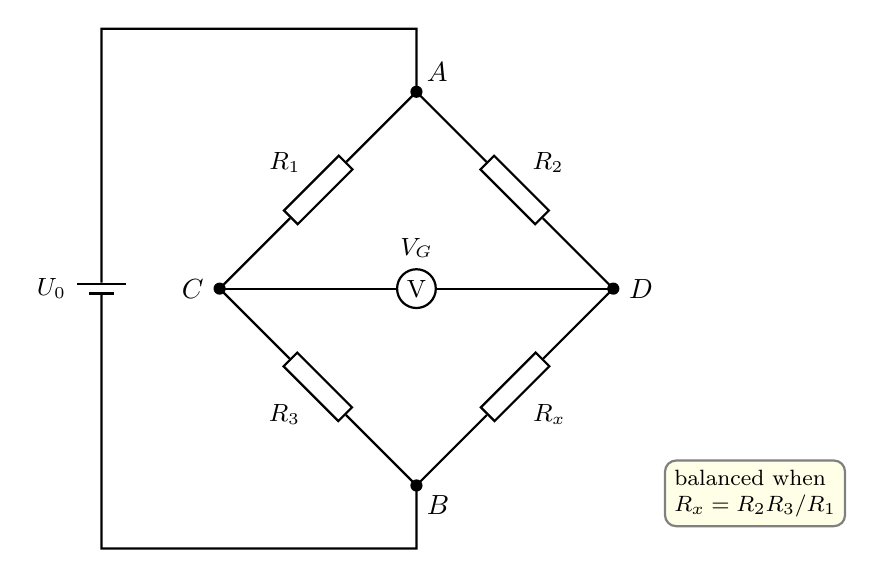
\begin{tikzpicture}[circuit ee IEC, thick, every info/.style={font=\small}]
  \coordinate (T) at (0,2.5);
  \coordinate (B) at (0,-2.5);
  \coordinate (L) at (-2.5,0);
  \coordinate (R) at (2.5,0);
  \draw (T) to [resistor={info'={$R_1$}}] (L) to [resistor={info'={$R_3$}}] (B);
  \draw (T) to [resistor={info={$R_2$}}] (R) to [resistor={info={$R_x$}}] (B);
  \draw (L) to [voltmeter={info={$V_G$}}] (R);
  \draw (T) -- (0,3.3) -- (-4,3.3) to [battery={info'={$U_0$}}] (-4,-3.3) -- (0,-3.3) -- (B);
  \foreach \p in {T,B,L,R} \fill (\p) circle (2.2pt);
  \node[above right] at (T) {$A$};
  \node[below right] at (B) {$B$};
  \node[left=2pt] at (L) {$C$};
  \node[right=2pt] at (R) {$D$};
  \node[align=left, font=\footnotesize, draw=gray, rounded corners, fill=yellow!10]
    at (4.3,-2.6) {balanced when\\$R_x = R_2 R_3 / R_1$};
\end{tikzpicture}
